\chapter{选择、遗传漂变与物种形成}\label{ch:g12:selection-drift-speciation}

1848 年，在一座工业城市附近捕获了一只黑色型的椒花蛾，
那里的每一棵树干都覆盖着煤烟；到 1895 年，几乎每一只
蛾都是黑色的。一个世纪后，煤烟消失，
树干重新变白，黑色型几乎绝迹。没有人培育
这些蛾，吃蛾的鸟类才是“分拣者”。前两
章讲述了变异如何产生；本章讨论的是变异在
\omterm{def:g12:selection-drift-speciation:population}{种群}中会发生什么——某些\omterm{def:g10:universal-dna:gene}{等位基因}如何变得常见，另一些
变得罕见，既有选择的作用，也有偶然的因素——以及一个\omterm{def:g12:selection-drift-speciation:population}{种群}
最终如何分化为两个\omterm{def:g10:biodiversity-scales:species}{物种}。

\section{种群及其等位基因}

\begin{definition}[种群，等位基因频率]\label{def:g12:selection-drift-speciation:population}
\emph{种群}\index{种群}是指同一\omterm{def:g10:biodiversity-scales:species}{物种}中生活在同一地点、彼此交配的
个体的集合。其遗传组成由各\omterm{def:g10:universal-dna:gene}{基因}的
\emph{等位基因频率}\index{等位基因频率}描述：对于有两个\omterm{def:g10:universal-dna:gene}{等位基因}的\omterm{def:g10:universal-dna:gene}{基因}，
其\omterm{def:g10:universal-dna:gene}{等位基因}为 $A$ 和 $a$，
全部拷贝中占比为 $p$ 的为 $A$，占比 $q = 1 - p$ 的为 $a$。
在这一尺度上，演化即
\omterm{def:g10:universal-dna:gene}{等位基因}频率从一代到下一代的变化。
\end{definition}

\begin{proposition}[无外力作用时的频率]\label{prop:g12:selection-drift-speciation:hw}
在一个大\omterm{def:g12:selection-drift-speciation:population}{种群}中，交配是随机的，没有任何\omterm{def:g10:universal-dna:gene}{等位基因}具有优势，
且不发生\omterm{def:g11:mutations:mutation}{突变}或迁移，则
\omterm{def:g12:selection-drift-speciation:population}{等位基因频率}逐代保持不变，且
各\omterm{def:g11:enzymes-and-phenotype:phenotype}{基因型}以如下比例出现：
\[
AA : Aa : aa = p^2 : 2pq : q^2 .
\]
这是参照状态：任何偏离该状态的现象，只要在
各世代中被观察到，即说明某一条件已不成立，
——即选择、偶然、迁移或\omterm{def:g11:mutations:mutation}{突变}正在起作用。
\end{proposition}
\begin{proof}
每个配子携带 $A$ 的概率为 $p$，携带 $a$ 的概率为
$q$；随机抽取两个配子，得到 $AA$ 的概率为 $p^2$，
$aa$ 的概率为 $q^2$，$Aa$ 的概率为 $pq + qp = 2pq$。统计
\omterm{def:g10:universal-dna:gene}{等位基因}：新一代中 $A$ 的拷贝所占比例为 $p^2 + \tfrac12 (2pq) =
p(p + q) = p$，频率保持不变。
\end{proof}

\begin{omfigure}
\begin{tikzpicture}[font=\small]
  \draw[thick] (0,0) rectangle (5,5);
  \fill[omDef!25] (0,1.5) rectangle (3.5,5);
  \fill[omProp!25] (3.5,1.5) rectangle (5,5);
  \fill[omProp!25] (0,0) rectangle (3.5,1.5);
  \fill[omThm!30] (3.5,0) rectangle (5,1.5);
  \draw (3.5,0) -- (3.5,5); \draw (0,1.5) -- (5,1.5);
  \node at (1.75,3.25) {$AA$: $p^2$}; \node at (4.25,3.25) {$Aa$: $pq$};
  \node at (1.75,0.75) {$Aa$: $pq$}; \node at (4.25,0.75) {$aa$: $q^2$};
  \node[anchor=south] at (1.75,5.1) {$A$，频率 $p$}; \node[anchor=south] at (4.25,5.1) {$a$，$q$};
  \node[anchor=east] at (-0.1,3.25) {$A$, $p$}; \node[anchor=east] at (-0.1,0.75) {$a$, $q$};
  \node[anchor=south, font=\small\itshape] at (2.5,5.6) {父方配子};
  \node[font=\small\itshape, rotate=90, anchor=south] at (-1.1,2.5) {母方配子};
  \node[anchor=west, align=left, text width=6cm] at (6,2.5) {当 $p = 0.7$ 且 $q = 0.3$ 时：$AA$ 占 49\%，$Aa$ 占 42\%，$aa$ 占 9\%。表现该隐性性状的个体占种群的 9\%，另有 42\% 的个体在默默携带该性状。};
\end{tikzpicture}

{\small 随机交配下的\omterm{def:g11:enzymes-and-phenotype:phenotype}{基因型}比例，以面积表示。
正方形的边为配子频率，四个矩形分别代表
四种\omterm{def:g11:enzymes-and-phenotype:phenotype}{基因型}。杂合子携带了稀有\omterm{def:g10:universal-dna:gene}{等位基因}的大部分拷贝。}
\end{omfigure}

\begin{example}[统计等位基因]\label{ex:g12:selection-drift-speciation:count}
在 1000 人中，490 人为 $AA$，420 人为 $Aa$，90 人为 $aa$。$a$ 的拷贝数为
$420 + 2 \times 90 = 600$，即 2000 个拷贝中的 600 个，故 $q = 0.3$ 且 $p = 0.7$——
且 1000 人中的\omterm{def:g11:enzymes-and-phenotype:phenotype}{基因型}人数恰好与 $p^2$、$2pq$、$q^2$ 相符：该
\omterm{def:g12:selection-drift-speciation:population}{种群}在该\omterm{def:g10:universal-dna:gene}{基因}上处于参照状态。一种\omterm{def:g11:genes-and-disease:genetic}{隐性}疾病
每 2500 名新生儿中有 1 人患病（$q^2 = 1/2500$），由此可得 $q = 1/50$，
携带者的比例 $2pq \approx 1/25$：正是
\cref{ch:g11:genes-and-disease}中的数字，由此推导得出。
\end{example}

\section{选择}

\begin{definition}[自然选择]\label{def:g12:selection-drift-speciation:selection}
\emph{自然选择}\index{自然选择}是指携带不同\omterm{def:g10:universal-dna:gene}{等位基因}的个体
之间在给定环境中的繁殖成效差异：携带某一\omterm{def:g10:universal-dna:gene}{等位基因}者平均
留下的后代比携带另一\omterm{def:g10:universal-dna:gene}{等位基因}者更多，该\omterm{def:g10:universal-dna:gene}{等位基因}的频率
逐代上升。被选择的是
整个个体——其生存、交配与
繁殖力——而
\omterm{def:g10:universal-dna:gene}{等位基因}则只是随之一同传递。
\end{definition}

\begin{proposition}[选择使频率朝一个方向变化]\label{prop:g12:selection-drift-speciation:direction}
若某\omterm{def:g10:universal-dna:gene}{等位基因}的携带者繁殖成效哪怕只略高，该\omterm{def:g10:universal-dna:gene}{等位基因}便会扩散；
若携带者繁殖成效较低，该\omterm{def:g10:universal-dna:gene}{等位基因}则变得罕见。变化
的方向由环境决定，环境改变时方向随之逆转；
速度取决于优势的大小，以及该\omterm{def:g10:universal-dna:gene}{等位基因}是否
在一个拷贝中即表达（\omterm{def:g11:genes-and-disease:genetic}{显性}，速度快），或仅在两个拷贝中才表达
（\omterm{def:g11:genes-and-disease:genetic}{隐性}，起初较慢，且从未被彻底消除，因其稀有的
拷贝隐藏于杂合子之中）。
\end{proposition}
\begin{proof}[证据]
椒花蛾的例子：鸟类捕食它们看到的蛾；在被煤烟覆盖的树干上，
浅色型更易被看到；在干净的树干上则是深色型更易被看到。深色\omterm{def:g10:universal-dna:gene}{等位基因}的频率
在五十年的污染期间由接近零升至 98\%，
而在四十年的清洁空气中又降至 10\% 以下，与树干的颜色同步变化。
\omterm{def:g11:antibiotic-resistance:antibiotic}{抗生素}抗性（见\cref{ch:g11:antibiotic-resistance}）：
仅耐药\omterm{def:g10:universal-dna:gene}{等位基因}的携带者能在存在该药物时繁殖。
乳糖酶持续性（见\cref{ch:g11:enzymes-and-phenotype}）：
该\omterm{def:g10:universal-dna:gene}{等位基因}恰在乳汁长期作为成人食物的地区最为常见，
已有数千年之久。在每个例子中，\omterm{def:g10:universal-dna:gene}{等位基因}的命运都紧随环境而变。
\end{proof}

\begin{omfigure}
\begin{tikzpicture}
\begin{axis}[
  width=0.88\linewidth, height=5.6cm,
  axis x line=bottom, axis y line=left,
  /pgf/number format/1000 sep={}, xmin=1840, xmax=2000, ymin=0, ymax=110,
  xlabel={年份}, ylabel={深色蛾（占捕获数的 \%）},
  xlabel style={font=\small, at={(axis description cs:0.5,-0.12)}, anchor=north},
  ylabel style={font=\small},
  tick label style={font=\small}, xtick={1850,1875,1900,1925,1950,1975,2000}, ytick={0,25,50,75,100},
  clip=false,
]
\addplot[thick, omThm, mark=*, mark size=1.3pt] coordinates
  {(1848,1) (1860,10) (1870,40) (1880,75) (1895,98) (1920,97) (1950,95) (1960,90) (1970,60) (1980,30) (1990,10) (1998,4)};
\draw[dashed, gray] (axis cs:1956,0) -- (axis cs:1956,105);
\node[font=\scriptsize, anchor=south] at (axis cs:1956,105) {清洁空气法规};
\end{axis}
\end{tikzpicture}

{\small 工业城市附近椒花蛾深色型的
频率（由博物馆标本与捕获记录取整）。频率上升与树干变黑同步，
下降则与树干被清洁同步。
环境逆转时，选择方向亦随之逆转。}
\end{omfigure}

\begin{omfigure}
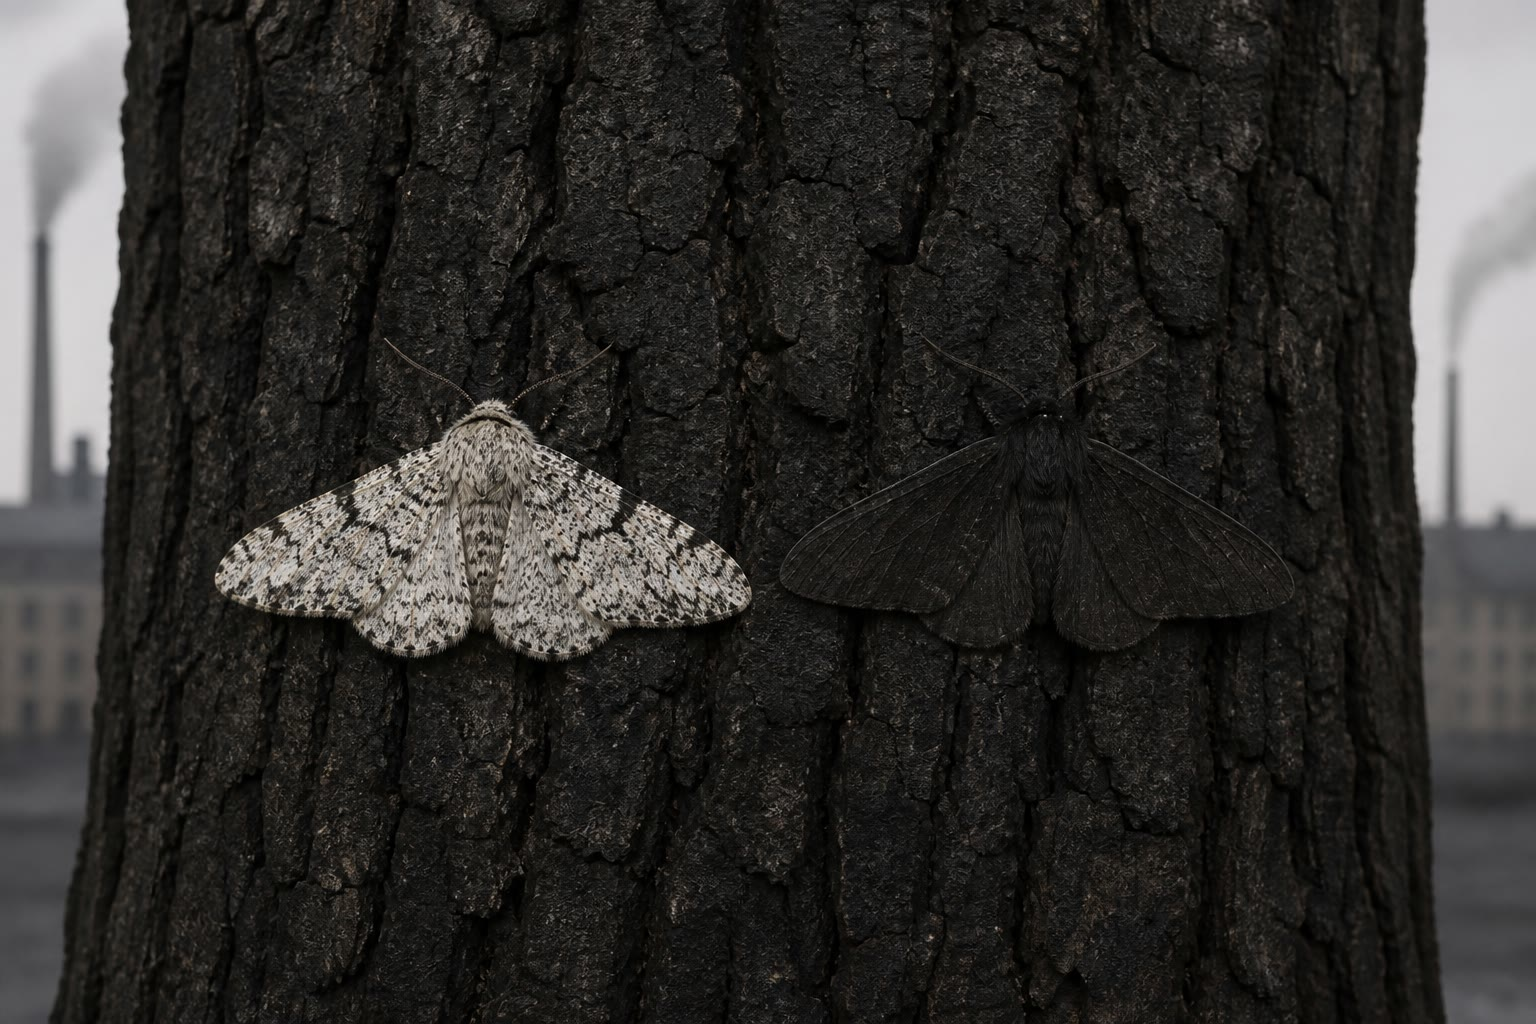
\includegraphics[width=0.6\linewidth]{images/book2/ai/g12-selection-peppered-moths.jpg}

{\small 椒花蛾的两种类型，停在被烟灰熏黑的树干上。
鸟类依靠视觉捕食：在这种树皮上，浅色型易被捕食，
深色型得以存活；在干净、长满地衣的树干上则恰好相反。}
\end{omfigure}

\begin{example}[异性选择]\label{ex:g12:selection-drift-speciation:sexual}
孔雀的尾羽使它飞行变慢，也更容易被捕食者发现，但它仍被保留下来，
因为雌孔雀总是选择尾羽最大、最规整的雄性：能使尾羽更出色的\omterm{def:g10:universal-dna:gene}{等位基因}，
无论它在生存上付出多大代价，都会更频繁地传递下去。
\emph{性选择}——即配偶的选择——
造就了动物的装饰、歌声与争斗，
并能把某一性状推向一个方向，
而仅凭生存选择永远不会朝这个方向发展。
\end{example}

\section{机遇：遗传漂变}

\begin{proposition}[遗传漂变]\label{prop:g12:selection-drift-speciation:drift}
在任何有限大小的\omterm{def:g12:selection-drift-speciation:population}{种群}中，一代的\omterm{def:g10:universal-dna:gene}{等位基因}是上一代的一个随机样本：
哪些个体恰好繁殖，其配子恰好携带哪些\omterm{def:g10:universal-dna:gene}{等位基因}，
都受机遇影响而波动。
因此，\omterm{def:g12:selection-drift-speciation:population}{等位基因频率}会逐代随机游移，
无需任何优势参与其中——这就是\emph{遗传漂变}\index{遗传漂变}。
\omterm{def:g12:selection-drift-speciation:population}{种群}越小，游移越大；在小\omterm{def:g12:selection-drift-speciation:population}{种群}中，
某一\omterm{def:g10:universal-dna:gene}{等位基因}仅凭机遇，便可能在数代之内丢失，或达到 100\%，
无论它本身的价值如何。
\end{proposition}
\begin{proof}[证据]
由少数个体建立的\omterm{def:g12:selection-drift-speciation:population}{种群}——例如被一小群鸟定居的岛屿，
或由几十名移民建立的人类群体——携带的是源\omterm{def:g12:selection-drift-speciation:population}{种群}\omterm{def:g10:universal-dna:gene}{等位基因}的一个失真样本：
某一罕见疾病的\omterm{def:g10:universal-dna:gene}{等位基因}在其中可能很常见，
而源\omterm{def:g12:selection-drift-speciation:population}{种群}的大部分多样性则缺失。
曾经历仅剩极少数幸存者这一\emph{瓶颈}的\omterm{def:g10:biodiversity-scales:species}{物种}（如
\cref{ch:g10:biodiversity-scales}中的猎豹，以及 1890 年仅剩二十只的北方象海豹），
即便数量恢复到数千只，
今天仍几乎没有\omterm{def:g10:biodiversity-scales:biodiversity}{遗传多样性}。
在实验室中，许多从相同频率出发的小型重复\omterm{def:g12:selection-drift-speciation:population}{种群}，
在几代之内便向各个方向分散，
而大\omterm{def:g12:selection-drift-speciation:population}{种群}则保持稳定。
\end{proof}

\begin{omfigure}
\begin{tikzpicture}
\begin{axis}[
  width=0.88\linewidth, height=5.8cm,
  axis x line=bottom, axis y line=left,
  xmin=0, xmax=20, ymin=0, ymax=1.05,
  xlabel={世代}, ylabel={等位基因 $A$ 的频率},
  xlabel style={font=\small, at={(axis description cs:0.5,-0.12)}, anchor=north},
  ylabel style={font=\small},
  tick label style={font=\small}, xtick={0,5,10,15,20}, ytick={0,0.25,0.5,0.75,1},
  legend style={at={(0.5,-0.3)}, anchor=north, legend columns=2, font=\small, draw=none},
]
\addplot[thick, omThm] coordinates {(0,0.5) (1,0.55) (2,0.6) (3,0.5) (4,0.65) (5,0.7) (6,0.6) (7,0.75) (8,0.85) (9,0.8) (10,0.9) (11,0.95) (12,1) (13,1) (14,1) (15,1) (16,1) (17,1) (18,1) (19,1) (20,1)};
\addplot[thick, omThm!60] coordinates {(0,0.5) (1,0.4) (2,0.45) (3,0.3) (4,0.35) (5,0.25) (6,0.3) (7,0.2) (8,0.1) (9,0.15) (10,0.05) (11,0.1) (12,0) (13,0) (14,0) (15,0) (16,0) (17,0) (18,0) (19,0) (20,0)};
\addplot[thick, omThm!35] coordinates {(0,0.5) (1,0.45) (2,0.55) (3,0.6) (4,0.5) (5,0.4) (6,0.45) (7,0.55) (8,0.6) (9,0.7) (10,0.65) (11,0.55) (12,0.5) (13,0.6) (14,0.65) (15,0.75) (16,0.7) (17,0.8) (18,0.75) (19,0.85) (20,0.8)};
\addplot[thick, omDef] coordinates {(0,0.5) (1,0.51) (2,0.49) (3,0.5) (4,0.52) (5,0.51) (6,0.5) (7,0.49) (8,0.48) (9,0.49) (10,0.5) (11,0.51) (12,0.52) (13,0.51) (14,0.5) (15,0.5) (16,0.49) (17,0.5) (18,0.51) (19,0.5) (20,0.5)};
\legend{三个大小为 20 的种群, 一个大小为 5000 的种群}
\end{axis}
\end{tikzpicture}

{\small 对一个中性\omterm{def:g10:universal-dna:gene}{等位基因}的模拟漂变，初始频率为 50\%。
在 20 个个体的\omterm{def:g12:selection-drift-speciation:population}{种群}中，它会在约十二代之内被固定或丢失，
且每次方向都不同；在 5000 个个体的\omterm{def:g12:selection-drift-speciation:population}{种群}中，
它几乎不动。}
\end{omfigure}

\begin{example}[奠基者效应]\label{ex:g12:selection-drift-speciation:founder}
一个岛屿群落由几十名移民建立，其中一人携带某种罕见眼疾的\omterm{def:g10:universal-dna:gene}{等位基因}。
十代之后，该\omterm{def:g10:universal-dna:gene}{等位基因}在群落中的频率为十分之一——是大陆数值的一百倍——
因为三十名奠基者中已有一名携带者，占全部拷贝的 1.7\%，
而小型孤立\omterm{def:g12:selection-drift-speciation:population}{种群}中的漂变又使其进一步增加。
该\omterm{def:g10:universal-dna:gene}{等位基因}并不带来任何优势；
它的常见程度纯属偶然，
取决于谁登上了那条船。
\end{example}

\begin{method}[选择还是漂变？]\label{met:g12:selection-drift-speciation:which}
面对\omterm{def:g12:selection-drift-speciation:population}{等位基因频率}的变化时：
\begin{enumerate}
  \item 估计\omterm{def:g12:selection-drift-speciation:population}{种群}的大小：\omterm{def:g12:selection-drift-speciation:population}{种群}低于几百个个体时，漂变作用很强，
        \omterm{def:g12:selection-drift-speciation:population}{种群}达到数百万个体时则可忽略。
  \item 寻找是否存在与环境变化相一致的方向（选择），
        或是否呈随机游走（漂变）。重复\omterm{def:g12:selection-drift-speciation:population}{种群}朝同一方向移动，
        表明存在选择；朝不同方向移动，
        则说明是漂变。
  \item 寻找将该\omterm{def:g10:universal-dna:gene}{等位基因}与生存或繁殖相联系的机制；
        若找不到这样的机制，则应怀疑是漂变。
  \item 注意两者可同时作用：选择设定趋势，
        漂变增加噪声，在小\omterm{def:g12:selection-drift-speciation:population}{种群}中，噪声可能淹没
        这一趋势。
\end{enumerate}
\end{method}

\section{从种群到物种}

\begin{proposition}[物种形成]\label{prop:g12:selection-drift-speciation:speciation}
同一\omterm{def:g10:biodiversity-scales:species}{物种}的两个\omterm{def:g12:selection-drift-speciation:population}{种群}，若停止\omterm{def:g10:universal-dna:gene}{基因}交流——被地理、行为或时间上的隔离所分开——便会各自演化：
每个\omterm{def:g12:selection-drift-speciation:population}{种群}积累自己的\omterm{def:g11:mutations:mutation}{突变}，
受自身环境选择，
并沿自己的方向漂变。
当两个\omterm{def:g12:selection-drift-speciation:population}{种群}的分化已达到一定程度，
即使它们再次相遇，个体之间也不再能杂交，或只产生不育后代，
原来的一个\omterm{def:g10:biodiversity-scales:species}{物种}便变成了两个\omterm{def:g10:biodiversity-scales:species}{物种}。
\emph{物种形成}\index{物种形成}即这一过程；它通常需要数千至数百万代，
不过\omterm{prop:g12:diversification-of-life:polyploidy}{多倍体}化（\cref{ch:g12:diversification-of-life}）可在一代之内实现。
\end{proposition}
\begin{proof}[证据]
岛屿：加拉帕戈斯群岛的每个岛上都有自己的雀类，
它们源自大陆上的一个\omterm{def:g10:biodiversity-scales:species}{物种}，与邻近岛屿的雀类关系最近。
湖泊：一种祖先慈鲷鱼在非洲某一湖泊中，
短短几十万年间分化出数百个\omterm{def:g10:biodiversity-scales:species}{物种}，
它们因栖息地不同，以及雌鱼对雄鱼颜色的选择而彼此分隔。
环状\omterm{def:g10:biodiversity-scales:species}{物种}：一种海鸥的\omterm{def:g12:selection-drift-speciation:population}{种群}环绕北极分布，
每个\omterm{def:g12:selection-drift-speciation:population}{种群}都与相邻\omterm{def:g12:selection-drift-speciation:population}{种群}杂交，直至绕行一周，
两端在欧洲相遇时已成为互不杂交的类型——一条正在形成中的
\omterm{def:g10:biodiversity-scales:species}{物种}界限。而近期才分化的\omterm{def:g10:biodiversity-scales:species}{物种}，
如北极熊与棕熊，仍偶尔能产生可育的杂种：
\omterm{def:g10:biodiversity-scales:species}{物种}界限本质上是程度问题。
\end{proof}

\begin{omfigure}
\begin{tikzpicture}[font=\small, >=Stealth]
  % one population
  \draw[thick, fill=omDef!12] (0,0) ellipse (1.4 and 0.8);
  \node at (0,0) {一个种群};
  \draw[->, thick] (1.6,0) -- (2.6,0) node[midway, above, font=\scriptsize, align=center] {屏障 \\ 出现};
  % two separated
  \draw[thick, fill=omDef!12] (4.0,0.9) ellipse (1.2 and 0.6); \node at (4.0,0.9) {种群 1};
  \draw[thick, fill=omDef!12] (4.0,-0.9) ellipse (1.2 and 0.6); \node at (4.0,-0.9) {种群 2};
  \draw[very thick, gray] (2.7,0) -- (5.3,0);
  \draw[->, thick] (5.5,0) -- (6.5,0) node[midway, above, font=\scriptsize, align=center] {分别 \\ 演化};
  % diverged
  \draw[thick, fill=omMeth!15] (7.9,0.9) ellipse (1.2 and 0.6); \node at (7.9,0.9) {突变组 1};
  \draw[thick, fill=omThm!15] (7.9,-0.9) ellipse (1.2 and 0.6); \node at (7.9,-0.9) {突变组 2};
  \node[font=\scriptsize, align=center] at (7.9,0.0) {各自选择，\\ 各自漂变};
  \draw[->, thick] (9.3,0) -- (10.3,0) node[midway, above, font=\scriptsize, align=center] {屏障 \\ 消失};
  % two species
  \draw[thick, fill=omMeth!15] (11.6,0.7) ellipse (1.1 and 0.55); \node at (11.6,0.7) {物种 1};
  \draw[thick, fill=omThm!15] (11.6,-0.7) ellipse (1.1 and 0.55); \node at (11.6,-0.7) {物种 2};
  \node[font=\scriptsize, align=center] at (11.6,0.0) {不再杂交};
\end{tikzpicture}

{\small 隔离导致的\omterm{prop:g12:selection-drift-speciation:speciation}{物种形成}。屏障将一个\omterm{def:g12:selection-drift-speciation:population}{种群}分开；每一
半个\omterm{def:g12:selection-drift-speciation:population}{种群}各自独立演化；当它们再次相遇时，二者已不再
杂交。屏障可以是海峡、山脉、
栖息地的改变，或交配中的偏好。}
\end{omfigure}

\begin{proposition}[重审物种]\label{prop:g12:selection-drift-speciation:concept}
\omterm{def:g10:biodiversity-scales:species}{物种}是指一个\omterm{def:g12:selection-drift-speciation:population}{种群}，或一组\omterm{def:g12:selection-drift-speciation:population}{种群}，其成员彼此杂交，
并在遗传上与其他此类集合相互隔离——这一定义
对大多数动植物在某一时刻都适用，但存在边界：正在分开的\omterm{def:g12:selection-drift-speciation:population}{种群}、
仍会杂交的\omterm{def:g10:biodiversity-scales:species}{物种}、
以及无性繁殖的生物。
\omterm{def:g10:biodiversity-scales:species}{物种}并非固定的类型，而是时间中的一条谱系：一个\omterm{def:g12:selection-drift-speciation:population}{种群}
被隔离时它便开始，只要其成员仍相互杂交便持续存在，
并因灭绝或分裂为新\omterm{def:g10:biodiversity-scales:species}{物种}而终结。
今天存活的\omterm{def:g10:biodiversity-scales:species}{物种}是一棵树的末梢，其分支
正是\cref{ch:g12:phylogenetic-trees}的研究对象。
\end{proposition}
\admitted

\begin{remark}[进化的综合]\label{rem:g12:selection-drift-speciation:assembled}
\omterm{def:g11:mutations:mutation}{突变}与\omterm{def:g10:universal-dna:gene}{基因}重组提供变异；重复、转移、
多倍化、调控与\omterm{def:g12:diversification-of-life:symbiosis}{共生}提供更多变异；\omterm{def:g12:selection-drift-speciation:selection}{自然选择}依环境筛选，
\omterm{prop:g12:selection-drift-speciation:drift}{遗传漂变}则凭机遇；隔离使\omterm{def:g12:selection-drift-speciation:population}{种群}分化直至成为\omterm{def:g10:biodiversity-scales:species}{物种}，灭绝则使其消亡。
这些步骤皆无目标，也不预见未来；
合起来，经过化石记录所载的
四十亿年，它们共同产生了
\cref{ch:g10:biodiversity-scales}中的多样性。命名这些步骤
及其相互作用的理论，即演化论；本年的每一章，
都是它的一份证据。
\end{remark}

\section{练习}

\begin{exercise}[$\star$]\label{exo:g12:selection-drift-speciation:1}
定义\omterm{def:g12:selection-drift-speciation:population}{等位基因频率}，并求出
参考状态下 $p = 0.8$ 的\omterm{def:g12:selection-drift-speciation:population}{种群}\omterm{def:g11:enzymes-and-phenotype:phenotype}{基因型}比例。
\end{exercise}

\begin{exercise}[$\star$]\label{exo:g12:selection-drift-speciation:2}
定义\omterm{def:g12:selection-drift-speciation:selection}{自然选择}和\omterm{prop:g12:selection-drift-speciation:drift}{遗传漂变}，
并说明二者的本质区别。
\end{exercise}

\begin{exercise}[$\star$]\label{exo:g12:selection-drift-speciation:3}
由蛾类图读出深色型在 1880 年和
1980 年的频率，并说出各自背后的环境变化。
\end{exercise}

\begin{exercise}[$\star$]\label{exo:g12:selection-drift-speciation:4}
为什么在小\omterm{def:g12:selection-drift-speciation:population}{种群}中\omterm{prop:g12:selection-drift-speciation:drift}{遗传漂变}的作用更大？
\end{exercise}

\begin{exercise}[$\star$]\label{exo:g12:selection-drift-speciation:5}
一个\omterm{def:g12:selection-drift-speciation:population}{种群}要分化为两个\omterm{def:g10:biodiversity-scales:species}{物种}，需要什么条件？
\end{exercise}

\begin{exercise}[$\star\star$]\label{exo:g12:selection-drift-speciation:6}
某\omterm{def:g12:selection-drift-speciation:population}{种群}共 500 个个体，其中 320 个为 $AA$，160 个为 $Aa$，
20 个为 $aa$。求 $p$ 和 $q$，再求参考状态下的
期望\omterm{def:g11:enzymes-and-phenotype:phenotype}{基因型}个体数，并加以比较。
\end{exercise}

\begin{exercise}[$\star\star$]\label{exo:g12:selection-drift-speciation:7}
一个\omterm{def:g11:genes-and-disease:genetic}{隐性}\omterm{def:g10:universal-dna:gene}{等位基因}的频率为 0.01。该\omterm{def:g12:selection-drift-speciation:population}{种群}中有多大比例
表现出\omterm{def:g11:genes-and-disease:genetic}{隐性}性状，又有多大比例携带该\omterm{def:g10:universal-dna:gene}{等位基因}却
不表现出来？为什么针对该性状的选择
很难淘汰这一\omterm{def:g10:universal-dna:gene}{等位基因}？
\end{exercise}

\begin{exercise}[$\star\star$]\label{exo:g12:selection-drift-speciation:8}
由漂变图可知，在两个到达两端的小\omterm{def:g12:selection-drift-speciation:population}{种群}中，
该\omterm{def:g10:universal-dna:gene}{等位基因}分别经过多少代被固定或丢失？
而第三个\omterm{def:g12:selection-drift-speciation:population}{种群}为何没有？
\end{exercise}

\begin{exercise}[$\star\star$]\label{exo:g12:selection-drift-speciation:9}
解释椒花蛾的深色\omterm{def:g10:universal-dna:gene}{等位基因}为何在
煤烟弥漫的数十年间没有达到 100\%，
并利用生活和繁殖于乡村的蛾加以说明。
\end{exercise}

\begin{exercise}[$\star\star$]\label{exo:g12:selection-drift-speciation:10}
二十只海豹经历瓶颈效应后存活下来；该\omterm{def:g10:biodiversity-scales:species}{物种}现今数量为 100\,000 只，
但几乎没有\omterm{def:g10:biodiversity-scales:biodiversity}{遗传多样性}。用\omterm{prop:g12:selection-drift-speciation:drift}{遗传漂变}加以解释。
\end{exercise}

\begin{exercise}[$\star\star$]\label{exo:g12:selection-drift-speciation:11}
运用\cref{met:g12:selection-drift-speciation:which}分析两种情形：一是
新捕食者出现后，十个相互隔离的湖泊\omterm{def:g12:selection-drift-speciation:population}{种群}中同时上升的一个\omterm{def:g10:universal-dna:gene}{等位基因}；
二是某一\omterm{def:g10:universal-dna:gene}{等位基因}在
由三十只鸟组成的岛屿\omterm{def:g12:selection-drift-speciation:population}{种群}中达到 80\%。
\end{exercise}

\begin{exercise}[$\star\star\star$]\label{exo:g12:selection-drift-speciation:12}
在一个疟疾流行的地区，镰刀型\omterm{def:g10:universal-dna:gene}{等位基因}的频率为 0.15，
尽管 $aa$ 个体的儿童很少能存活。利用\omterm{def:g11:enzymes-and-phenotype:phenotype}{基因型}比例，
计算新生儿中 $AA$、$Aa$ 和 $aa$ 的比例，
并说明 $Aa$ 个体对疟疾的优势如何在
失去 $aa$ 个体的情况下使该\omterm{def:g10:universal-dna:gene}{等位基因}仍然常见。
\end{exercise}

\begin{exercise}[$\star\star\star$]\label{exo:g12:selection-drift-speciation:13}
同一湖泊中的两种丽鱼主要区别在于雄鱼的体色，
而每种雌鱼都选择自己的体色。在浑浊的水中，
颜色无法被看见，两者可以自由杂交。是什么使这两个\omterm{def:g10:biodiversity-scales:species}{物种}相互隔离，
以及浑浊水域中的情形说明这种分离
发生得有多晚？
\end{exercise}

\begin{exercise}[$\star\star\star$]\label{exo:g12:selection-drift-speciation:14}
试解释鸥的环状\omterm{def:g10:biodiversity-scales:species}{物种}为何说明\omterm{prop:g12:selection-drift-speciation:speciation}{物种形成}是渐进的，
以及在欧洲相遇的两端为何仍被称为
两个\omterm{def:g10:biodiversity-scales:species}{物种}。
\end{exercise}

\begin{exercise}[$\star\star\star$]\label{exo:g12:selection-drift-speciation:15}
“选择使生物变得更好。”请用一段话讨论：在什么方面更好、
在何处、与谁相比更好；
以及\omterm{prop:g12:selection-drift-speciation:drift}{遗传漂变}、性状逆转和性选择各增加了什么。
\end{exercise}

\section{问题：岛上的小鼠}

\begin{problem}[{周末问题——岛上小鼠种群：
计算其等位基因频率，追踪新捕食者的选择作用，
模拟一个小群体的遗传漂变，
并预见一个新物种的形成}]
\label{pb:g12:selection-drift-speciation:1}
在一个多岩石的岛上，小鼠携带一个毛色\omterm{def:g10:universal-dna:gene}{基因}，该\omterm{def:g10:universal-dna:gene}{基因}有两个\omterm{def:g10:universal-dna:gene}{等位基因}：$D$
（深色，\omterm{def:g11:genes-and-disease:genetic}{显性}）和 $d$（浅色）。对 2000 只小鼠的普查发现，\omterm{def:g11:enzymes-and-phenotype:phenotype}{基因型}为 $DD$ 的深色小鼠有 720 只，
深色 $Dd$ 的有 960 只，浅色 $dd$ 的有 320 只。

\medskip
\noindent\textbf{第一部分——当前的\omterm{def:g12:selection-drift-speciation:population}{种群}。}
\begin{enumerate}
  \item 通过计数拷贝，计算频率 $p$（\omterm{def:g10:universal-dna:gene}{等位基因} $D$ 的频率）和
        $q$（$d$ 的频率）。
  \item 计算参考状态下预期的各\omterm{def:g11:enzymes-and-phenotype:phenotype}{基因型}数目，
        并与普查数据相比较。该\omterm{def:g12:selection-drift-speciation:population}{种群}是否处于
        参考状态？
  \item 深色小鼠中，携带 $d$ 的比例是多少？
  \item 根据上一问的答案，解释为何将岛上所有浅色小鼠
        移除一代只会使 $q$ 略有降低。
        若剩余小鼠随机交配，计算移除后的新
        $q$ 值。
  \item 参考状态的四个条件中，哪一个在小岛上最可能不成立，
        产生何种后果？
\end{enumerate}

\medskip
\noindent\textbf{第二部分——捕食者到来。}
猫头鹰迁入该岛。在浅色岩石上，深色小鼠被看见并被捕食的频率
高出一倍：每一代中，一半深色小鼠在繁殖前死亡，
而所有浅色小鼠都存活下来。
\begin{enumerate}[resume]
  \item 以普查数据为起点，计算第一代中
        各\omterm{def:g11:enzymes-and-phenotype:phenotype}{基因型}能存活并繁殖的小鼠数目。
  \item 计算存活个体中的 $p$ 和 $q$。
  \item 若存活个体随机交配，计算下一代的\omterm{def:g11:enzymes-and-phenotype:phenotype}{基因型}比例，
        然后再次施加猫头鹰的捕食作用，
        并计算其存活个体中的 $q$。
  \item 再重复一次（保留两位有效数字），描述三代中
        $q$ 的变化趋势。
  \item 解释 $q$ 为何稳步上升，
        以及为何 $D$ 与同样选择作用下的\omterm{def:g11:genes-and-disease:genetic}{隐性}\omterm{def:g10:universal-dna:gene}{等位基因}不同，
        能够被完全消除。
\end{enumerate}

\medskip
\noindent\textbf{第三部分——一个由六只小鼠组成的群体。}
一场风暴把六只小鼠带到邻近的小岛：$DD$ 2 只，$Dd$ 3 只，$dd$ 1 只。
\begin{enumerate}[resume]
  \item 计算小群体中的 $q$，并与岛上的情况相比较。
  \item 在第一窝中，偶然只有两只 $DD$ 与一只 $Dd$ 繁殖。
        下一代中 $q$ 可能的取值是多少？
        该\omterm{def:g12:selection-drift-speciation:population}{种群}的变异发生了什么变化？
  \item 解释为何在小岛上，即使没有猫头鹰或任何优势，
        一个\omterm{def:g10:universal-dna:gene}{等位基因}也可能在几代之内消失。
  \item 小岛上没有猫头鹰。预测 $d$ 在那里的命运，
        并说明为何两个相邻的岛屿可以在没有适应性原因的情况下
        最终呈现不同的毛色。
  \item 写出该过程的名称，以及使其在该群体中起主导作用的
        群体特征。
\end{enumerate}

\medskip
\noindent\textbf{第四部分——一万年之后。}
隔离的小岛小鼠已经产生分化：体型更小，毛色更浅，
且繁殖季节不同。将它们与岛上小鼠一同置于实验室中时，
两者很少交配，即使产生的少数杂种也是不育的。
\begin{enumerate}[resume]
  \item 小岛上的小鼠是否为一个新\omterm{def:g10:biodiversity-scales:species}{物种}？请根据
        定义说明理由。
  \item 指出引发这一过程的隔离屏障，以及推动分化的
        两种机制。
  \item 两者的繁殖季节不同。解释这种差异一旦出现，
        如何加强隔离。
  \item 若小岛明天重新与岛屿相连，两者会否重新合并为
        一个\omterm{def:g12:selection-drift-speciation:population}{种群}？请区分第 17 题的情形与较早阶段
        （例如 100 年后）的情形。
  \item 给出结果：猫头鹰作用三代前后岛上 $d$ 的频率，
        小岛上 $d$ 的命运，
        及其起作用的过程，
        以及最终的\omterm{def:g10:biodiversity-scales:species}{物种}数目。
\end{enumerate}
\end{problem}
